\chapter{Методы экспериментальных исследований и получения образцов} \label{chapt2}

В главе описаны основные методы и методики исследования и синтеза соединений для систем Cu--As--S, Cu--Sb--S, Cu--As--Se и Cu--Sb--Se в стехиометрическом соотношении 3:1:3.
А именно: методы порошковой и монокристальной дифрактометрии, измерения и моделирования теплоёмкости, просвечивающей электронной микроскопии и измерения магнитной восприимчивости.
Также описаны условия проведения квантовомеханических расчётов.

В литературе широко обсуждаются методы получения синтетических образцов соединений из группы тетраэдрита--теннантита. Один из них позволяет сократить время синтеза и получить образец за одну итерацию --- методом ампульного синтеза из исходных чистых элементов.

Аттестация полученных образцов проводилась общепринятыми и хорошо апробированными методами порошковой дифрактометрии.

Использование методов магнитометрии и измерения теплоёмкости обусловлено высокой точностью измерения физических свойств и их чувствительностью к структуре.
Использованные в работе методики основаны на  Physical Property Measurement System (Quantum Design, США), которая отвечает всем современным требованиям научных исследований, широко применяется и развивается мировым научным сообществом.
Использование распространенной и современной системы PPMS позволяет сравнивать полученные результаты в контексте уже опубликованных данных для исследуемых соединений и получать оценку объективности результатов.
Другие чувствительные к структуре методы не были выбраны:
методы измерения электрических свойств и эффекта Холла не удалось применить ко всем исследуемым образцам, а метод электронного парамагнитного резонанса сложен в интерпретации и моделировании ввиду отсутствия актуальных структурных данных для всех исследуемых соединений.

\section{Методика синтеза трёхкомпонентных соединений из группы тетраэдрита--теннантита} \label{sect2_1}

Соединения из группы тетраэдрита--теннантита синтезированы из элементарных компонентов.
В качестве исходных материалов применяли реактивы высокой чистоты марки ОСЧ.

\begin{figure}[pt!]
  \begin{minipage}[ht]{0.99\linewidth}\centering
    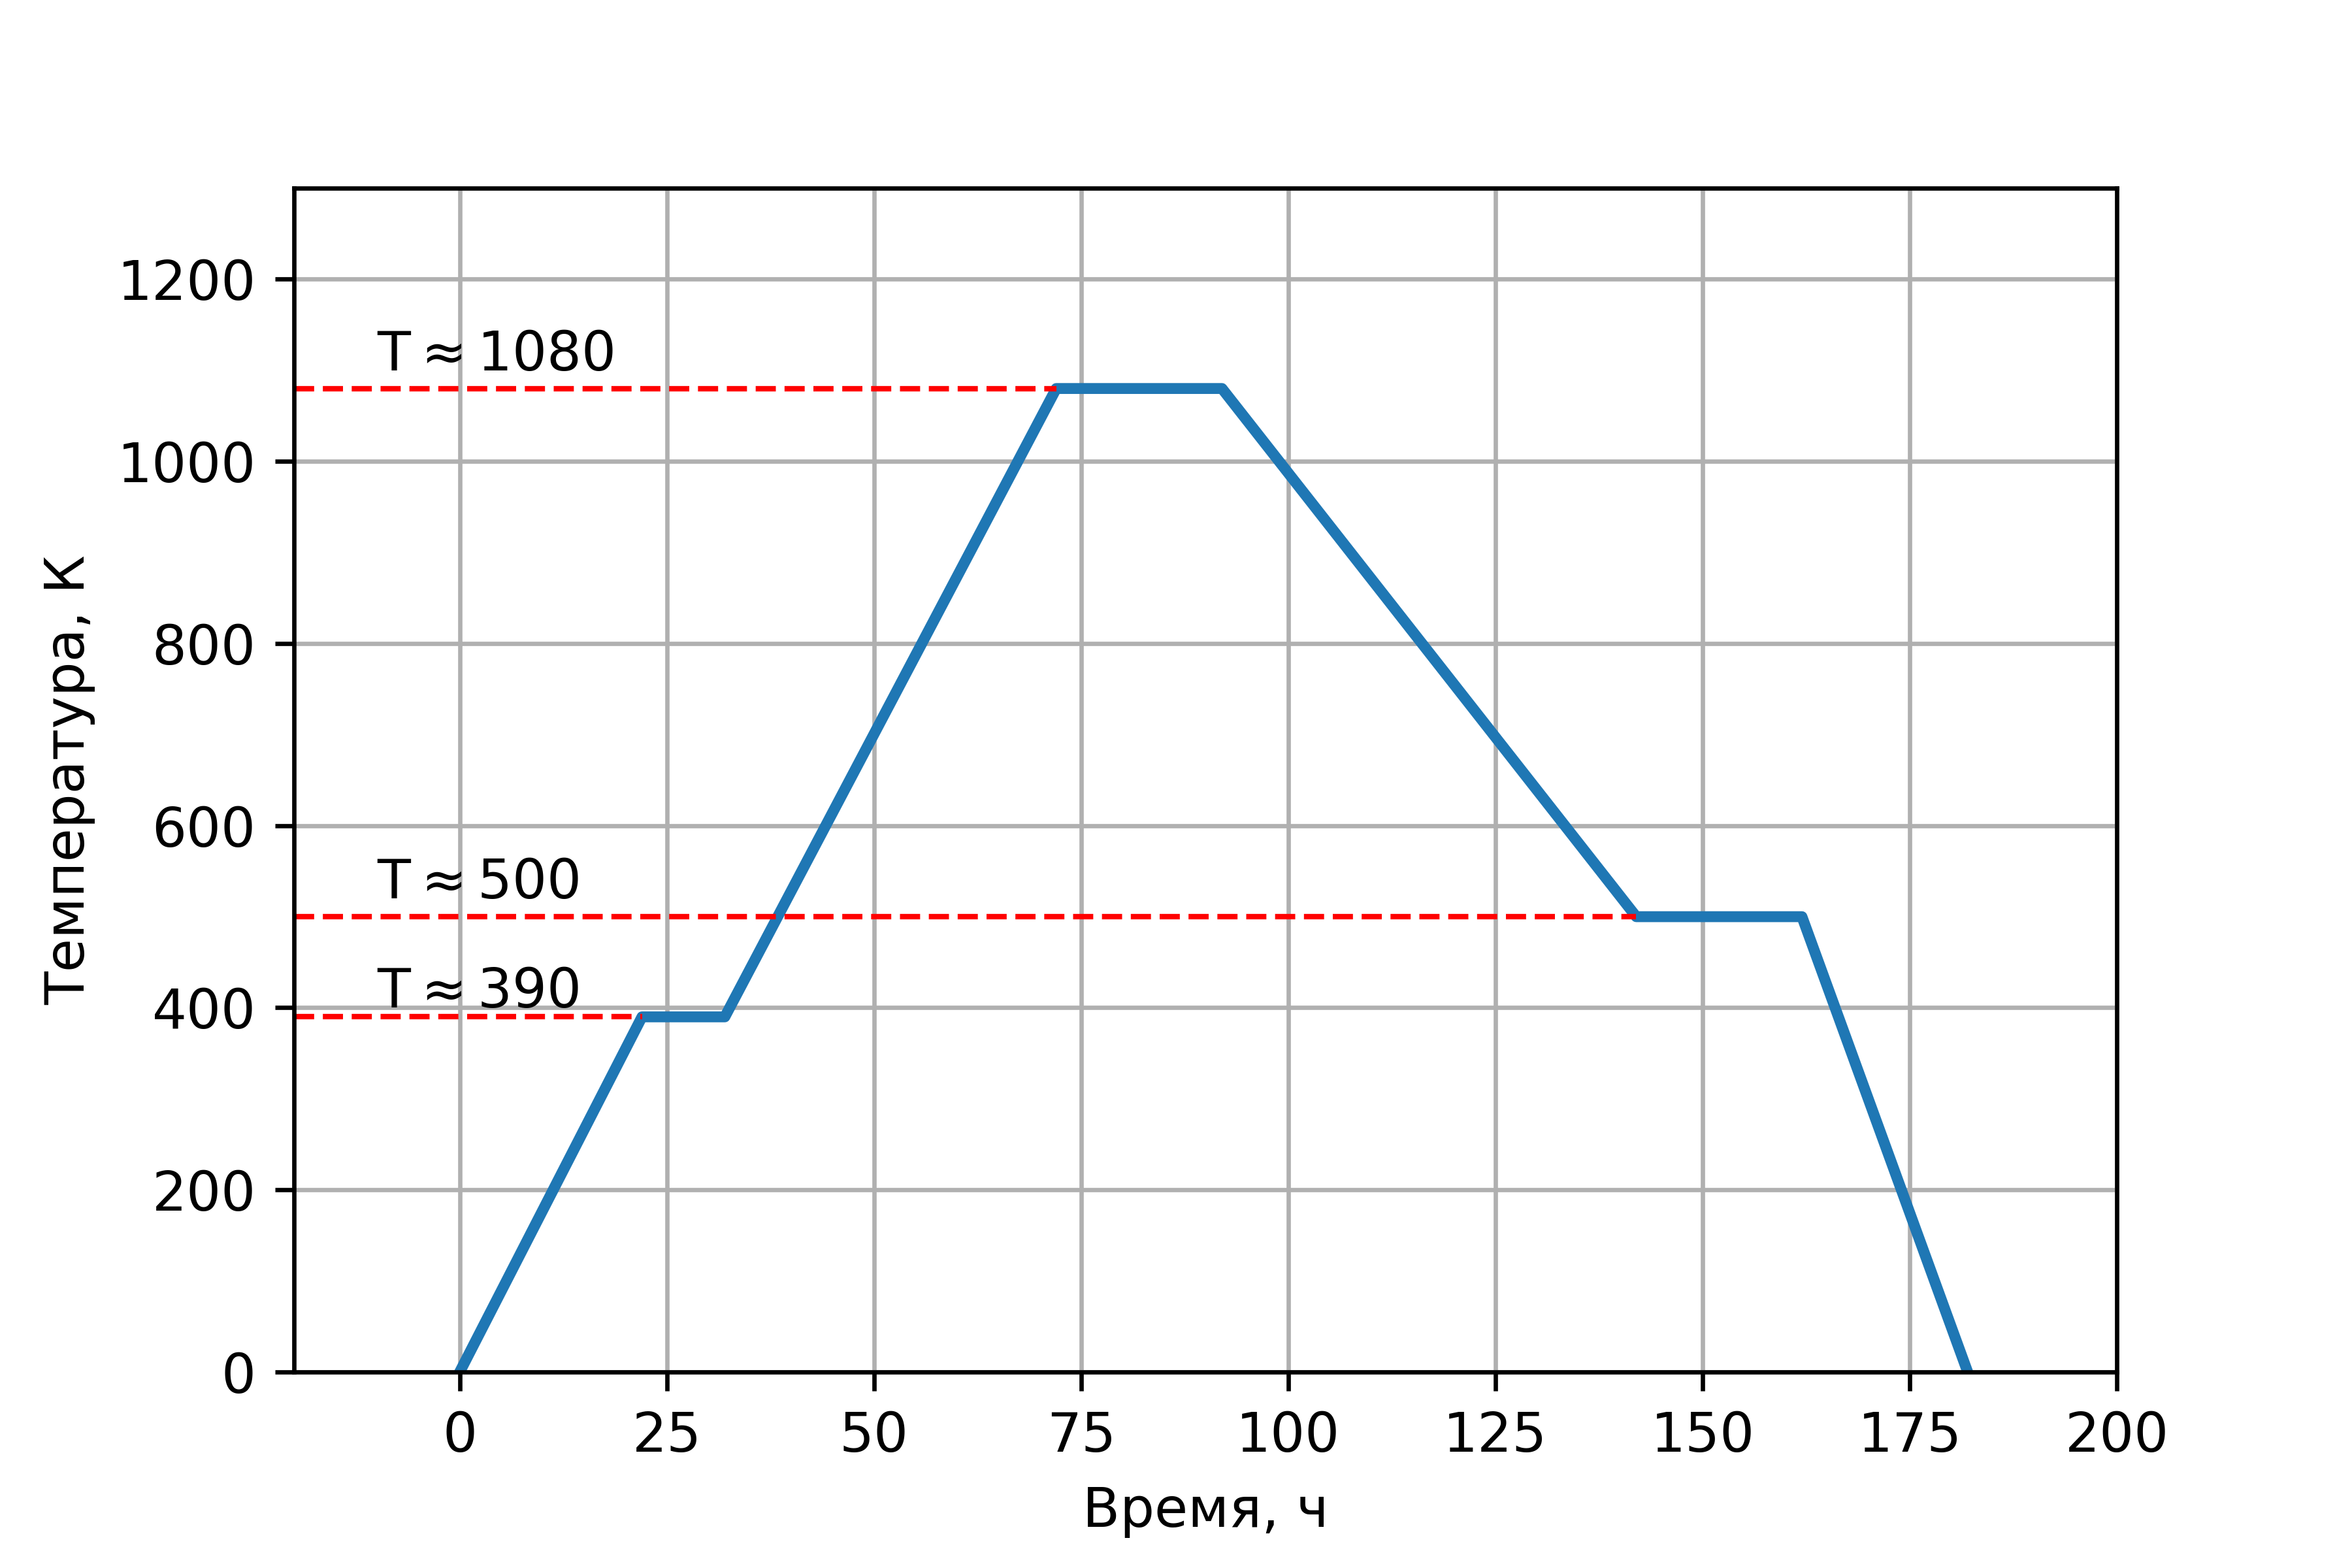
\includegraphics[width=0.99\linewidth]{5_synthesis}
  \end{minipage}
       \caption[Схема температурного режима синтеза соединений Cu\textsubscript{12}As\textsubscript{4}S\textsubscript{13} и Cu\textsubscript{12}Sb\textsubscript{4}S\textsubscript{13}]{Схема температурного режима синтеза соединений Cu\textsubscript{12}As\textsubscript{4}S\textsubscript{13} и Cu\textsubscript{12}Sb\textsubscript{4}S\textsubscript{13}(описание в тексте)}
    \label{img:figure3}
\end{figure}

Синтез соединений проводили в кварцевых ампулах при остаточном давлении 1$\cdot$10$^{-1}$~Па и заполненных обескислороженным аргоном или гелием при давлении 0.5$\cdot$10$^{5}$~Па. Очистку ампул проводили по схеме рекомендованной в \cite{156} с предварительной промывкой, травлением в азотной и фтористоводородной кислотах, промывкой дистиллированной водой и вакуумной сушкой в диапазоне температур от 900 до 1000~К и остаточном давлении 1$\cdot$10$^{-3}$~Па в течение 4--5~часов. Взвешивание исходных компонентов проводили на аналитических весах АВД--200 с точностью $\pm$5$\cdot$10$^{-5}$~г.
С целью компенсации ухода халькогена в газообразную фазу и обеспечения избыточного давления его паров в процессе синтеза навеску серы или селена делали с избытком (0.2--0.5\% по массе).
Для минерала cмитита показано\cite{181}, что избыточное содержание серы в таких количествах не выходит за пределы области гомогенности, но в то же время компенсирует уход халькогена в газообразную фазу и обеспечивает (вместе с давлением гелия или аргона) избыточное давление его паров в процессе синтеза, а также препятствует возникновению микропор в объеме синтезируемого соединения.
Точность определения температуры в~рабочей камере печи соответствовала 0,5~К при 600~К и 1~К при 1100~К (термопара платины и сплав платины с 10~\% родием использовалась для контроля температуры). Синтез проведен в~четыре этапа. Первый "--- медленное нагревание в~печи (10--15~часов) до~температуры, превышающей температуру плавления легколетучего компонента (серы или селена) на~10--30~К; второй "--- поддержание данной температуры 20--30~часов. Третий этап "--- увеличение температуры до~полного плавления образовавшегося в~ампуле вещества в течении 40--50~ч. и поддержание этой температуры постоянной 20--30 ч. Последний, четвертый этап  "--- понижение температуры до 2/3 от температуры плавления и отжиг соединения 30--40~ч.
 Пример схемы температурного режима представлен на рисунке \ref{img:figure3}. Образец Cu\textsubscript{12}As\textsubscript{4}S\textsubscript{13} после спекания дополнительно был подвергнут направленной перекристаллизации в~двухзонной печи по~методу Стокбаргера--Бриджмена. Часть образцов дополнительно была отожженна при~температуре 673 и 773~К в~течении 24~часов.
Перед отжигом образцы были перетерты в ступке и подвергнуты горячему прессованию.

\newpage
%============================================================================================================================
\section{Методы порошковой и монокристальной дифрактометрии} \label{sect2_2}
В этой главе описаны методы прецизионных дифракционных экспериментов. Все полученные образцы аттестованы на порошковом дифрактометре D8
Advance (Bruker, Германия) на Cu K$\alpha$ излучении.
Характеристическое излучение данного дифрактометра монохроматизируется зеркалом Гёбеля, в нем используются щели Соллера  для формирования нужного геометрического размера рентгеновского излучения. Порошкообразные образцы получены истиранием до гомогенного состояния. Рентгенофазовый анализ проведен методом порошка (Дебая--Шеррера) на образцах, которые  получены истиранием исходных спёченных образцов до гомогенного состояния в ступке. Дифрактограммы  обрабатывались в программном комплексе Jade 6 с использованием реферативной базы pdf2. Три соединения из синтезированных идентифицированы в кубической сингонии, одно --- в тетрагональной сингонии. Данные рентгенофазового анализа представлены в таблице \ref{xray_comp}.


\begin{table} [htbp]
\centering
\caption{Сводная таблица данных рентгенофазового анализа синтезированных соединений}%
	\label{xray_comp}% label всегда желательно идти после caption
    \renewcommand{\arraystretch}{1.5}
	\begin{tabular}{@{}@{\extracolsep{10pt}}llllllll@{}}
 \toprule     %%% верхняя линейка
     & &a,$\angstrom$  & b,$\angstrom$ & c,$\angstrom$  & $\alpha$,\textsuperscript{ $\circ$ }   & $\beta$,\textsuperscript{ $\circ$ } & $\gamma$,\textsuperscript{ $\circ$ }  \\ \midrule
Cu\textsubscript{12}As\textsubscript{4}S\textsubscript{13} & I$\overline{\! 4}$3m &\multicolumn{3}{c}{10.1439}  & \multicolumn{3}{c}{90}  \\ \hline
Cu\textsubscript{3}AsSe\textsubscript{3}                         & F$\overline{\! 4}$3m &\multicolumn{3}{c}{5.53}  & \multicolumn{3}{c}{90}     \\ \hline
Cu\textsubscript{12}Sb\textsubscript{4}S\textsubscript{13}  & I$\overline{\! 4}$3m &\multicolumn{3}{c}{10.30450}&\multicolumn{3}{c}{90}  \\ \hline
Cu\textsubscript{3}SbSe\textsubscript{3} & Pnma & 7.9865 & 10.6138 &6.837& \multicolumn{3}{c}{90} \\ \hline

 \bottomrule
\end{tabular}
\end{table}

Образец, полученный методом направленной перекристаллизации в~двухзонной печи по~методу Стокбаргера"--~Бриджмена, был подвергнут прецизионному дифракционному исследованию на монокристальном дифрактометре Xcalibur с 2d детектором CCD~EOS~S2 (Rigaku Oxford Diffraction). Образец представлял из себя шар диаметром от 200 до 300~мкм, изготовленный специальным образом из скола от монокристаллического образца, или скол от пластинки образца толщиной 0.3~мм. Исследовательское оборудование является особым научным прибором, который предназначен для высокоточных дифракционных экспериментов. Исследование проводилось при температурах 85, 115, 180, 250 и 293~К\cite{Dudka2016}. Температура определялась по детектору, который находился на сопле охлаждающей системы Cobra Plus. Хладагентом служил азот. Расстояние между соплом с хладагентом до образца составляло 7~мм.

Детектор CCD~EOS~S2 и гониометр были предварительно откалиброваны экспериментально\cite{Dudka2010} с использованием монокристалла Ca\textsubscript{3}TaGa\textsubscript{3}Si\textsubscript{2}O\textsubscript{14}\cite{Dudka2016_b}. Полученная калибровка повысила точность получаемых данных на 10~\%.

Сбор данных, обработка и учет поглощения проводился в программном комплексе  CrysAlisPro. Коррекция поглощения на форму образца проведена интегральным методом Гаусса. Уточнение структуры произведено в программе Jana2000\cite{Dusek2001}.



%Используемая система основана на дифрактометре HUBER--5042, выпущенном в 1999 году, который был модифицирован в 2015--2017 годах. Модификация заключена в оснащении современным компьютером, поддерживающим новые скоростные протоколы передачи данных.
%Обмен данных между дифрактометром и персональным компьютером основан на блоке PCIDCC5--P, который выполняет роль устройства определяющего время и количество импульсов.
%Шаговые моторы дифрактометра управляются через интерфейс стандарта RS232. Вакуум внутри бриллиевых емкостей, где помещается образец, поддерживается турбомолекулярным насосом TPS-compact (Agilent Technologies). Охлаждающая система состоит из двух независимых устройств: охлаждение рентгеновской трубки и гелиового охлаждения образца.
%Программное обеспечение позволяет удалённо управлять измерительным комплексом.



Во время прецизионных  экспериментов использовалось MoK\textsubscript{$\alpha$}"~излучение ($\lambda$ = 0,71069~${\angstrom}$, графитовый монохроматор). Сбор данных проводился c использованием 2d детектора. Максимальное значение составляло $\theta$\textsubscript{max} = 42\textsuperscript{$\circ$}.
Угловые положения образца задавались с точностью 0.001\textsuperscript{$\circ$}.
Исходный R"~фактор усреднения R\textsubscript{уср}(I) составил не более чем 0.054, R/R\textsubscript{w} = 0.033/0.053 и уточнение проведено не менее чем по 11026 рефлексам.
Величины остаточных пиков разностной электронной плотности составили $\pm\Delta$$\rho$ = +2.7/$-$1.6.
Погрешность в параметрах ячейки не превышала 0.0002~{$\angstrom$}.

Дополнительно был проведен эксперимент на CAD4 с точечным детектором при комнатной температуре и на образце в форме шара. Во время прецизионных экспериментов использовалось AgK\textsubscript{$\alpha$}"~излучение ($\lambda$ = 0,56083~${\angstrom}$, графитовый монохроматор). Сбор данных проводился при использовании точечного детектора по $\theta$/2$\theta$"~сканированию (c $\theta$\textsubscript{max} = 30\textsuperscript{$\circ$}).
Исходный R"~фактор усреднения R\textsubscript{уср}(I) составил не более чем  0.041, R/R\textsubscript{w} = 0.032/0.043 и уточнение проведено по 3509 рефлексам.
Величины остаточных пиков разностной электронной плотности составили $\pm\Delta$$\rho$ = +0.7/$-$0.9.
Погрешность в параметрах ячейки не превышала 0.0002~{$\angstrom$}.

\newpage
%============================================================================================================================
\section{Методы измерения и моделирования теплоёмкости} \label{sect2_4}
\subsection{Экспериментальное измерение теплоёмкости}\label{sect2_4_1}
Теплоёмкость синтезированных соединений измерена при помощи измерительного комплекса PPMS (Quantum Design,
США) в диапазоне температур от 2 до 350 К. Измерения проводились методом релаксации теплового
импульса\cite{Hwang_1997}. Измерительная установка представляет собой автономный комплекс с гелиевым криостатом замкнутого цикла. Данный метод основан на измерении времени релаксации теплового импульса. Преимущество метода заключается в том, что:
\begin{itemize}
\item Метод не критичен к размеру, форме образца и величине $\tau$\textsubscript{1}.

\item Метод позволяет измерять теплоёмкость в адиабатических и неадиабатических циклах в широком диапазоне температур.

\item Теплоёмкость автоматически определяется из прямых измерений  $\tau$\textsubscript{1} и $\tau$\textsubscript{2}.

\item Существует возможность ввести корректировки на учёт погрешности вызванной нагреванием подложки, на которой находится образец.

\item Тепловое переключение не нужно.

\item Эффекты, связанные с $\tau$\textsubscript{2}, учитываются должным образом.
\end{itemize}


\begin{equation}
  \label{eq:equation2.2}
\begin{cases}
    P(t)=c'\frac{dT'}{dt}+\lambda_{s}(T'-T)+\lambda_{l}(T'-T_{0}) \\
    0 = c\frac{dT}{dt}+\lambda_{s}(T-T')
\end{cases} ,
\end{equation}

где c и T теплоёмкость и температура образца соответственно, с$'$ и T$'$ "--- теплоёмкость и температура держателя образца, P(t) "--- мощность, T\textsubscript{0} "--- температура теплоотвода, $\lambda$\textsubscript{l} "--- значение теплопроводности между теплоотводом и держателем образца, $\lambda$\textsubscript{s} "--- теплопроводность между образцом и держателем образца. Данное представление имеет место только в случае, если нагреватель и сенсор достаточно хорошо прикреплены к держателю образца и теплопроводность образца много больше, чем теплопроводности $\lambda$\textsubscript{l} и $\lambda$\textsubscript{s}.
Также допускается, что $\lambda$\textsubscript{l}, $\lambda$\textsubscript{s}, с и с$'$ температурно независимы от слабого изменения температуры.

Из системы уравнений \ref{eq:equation2.2} избавимся от T и учтем что P(t)~$=$~0 и dt$_{1}^{2}$/dt$^2$~$\cong$~0 получаем:

\begin{equation}
  \label{eq:equation2_4}
\cfrac{сc'}{\lambda_{s}}\cfrac{d^2T_1}{t^2}+\Bigg(c'+c+c\cfrac{\lambda_{l}}{\lambda_{s}}\Bigg)\cfrac{dT_1}{dt}+\lambda_{l}T_l=\lambda_{l}T_0.
\end{equation}


После рассуждений и математических преобразований в \cite{Hwang_1997} получаем выражение для теплоёмкости:

\begin{equation}
  \label{eq:equation2_3}
c'+c\cong c'+c\cfrac{\lambda_{l}}{\lambda_{s}}=\cfrac{P(t_{h})}{\frac{dT}{dt}\big|_{t=t_{h}}-\frac{dT}{dt}\big|_{t=t_{b}}}.
\end{equation}

Таким образом, измеряя значения времени регистрации, зная величину теплового импульса и времени нагрева, находим значение теплоёмкости исследуемого образца.

Экспериментальная схема измерения теплоёмкости на измерительном комплексе Quantum Design PPMS представлена на рисунке \ref{img:figure2}. Образец (4) помещается на платформу (5), которая висит в вакууме на тонких медных проводах (1). Эти тонкие медные провода служат теплоотводом (2) для теплоты, полученной от нагревателей (3 и 7). Образец крепится специальным гелем (6), обладающим постоянной теплоёмкостью в широком диапазоне температур.
\begin{figure}[ht]
  \begin{minipage}[ht]{0.99\linewidth}\centering
    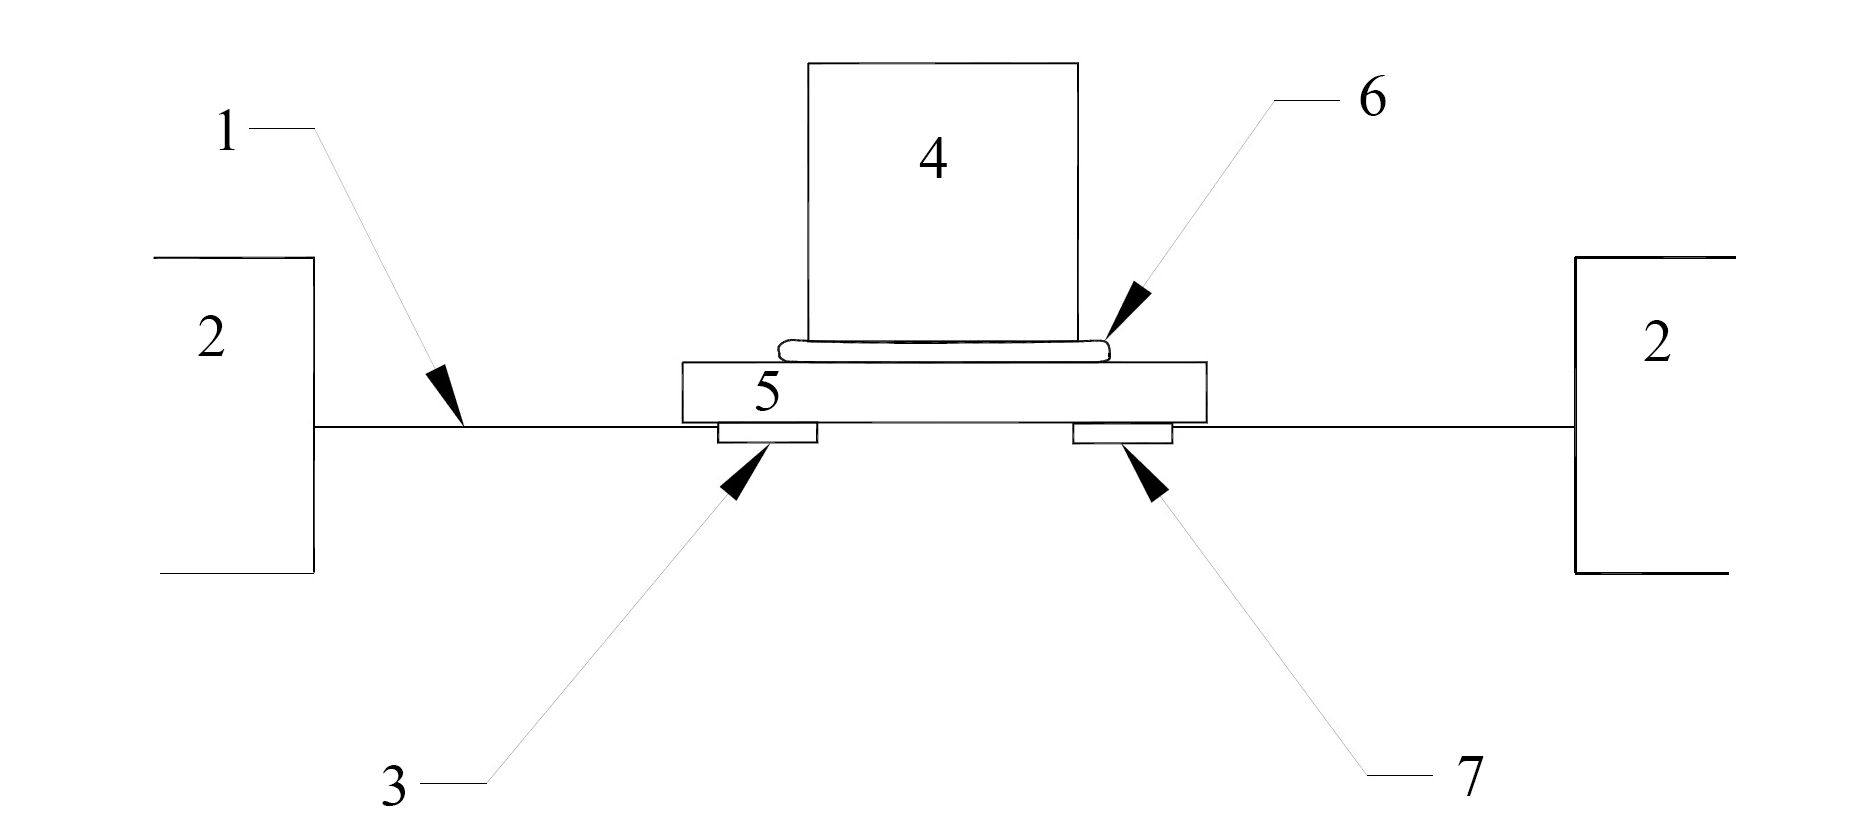
\includegraphics[width=0.99\linewidth]{4_heat_capacity_scheme}
  \end{minipage}
       \caption[Схематическое изображение схемы измерения теплоёмкости на измерительном комплексе Quantum Design PPMS]{Схематическое изображение схемы измерения теплоёмкости на измерительном комплексе Quantum Design PPMS. 1 "--- медные провода, 2 "--- теплоотвод, 3 и 7 "--- нагреватель, 4 "--- образец, 5 "--- платформа образца, 6 "--- теплопроводящий гель (описание дано в тексте)}
    \label{img:figure2}
\end{figure}

\begin{figure}[p!]
  \begin{minipage}[ht]{0.99\linewidth}\centering
    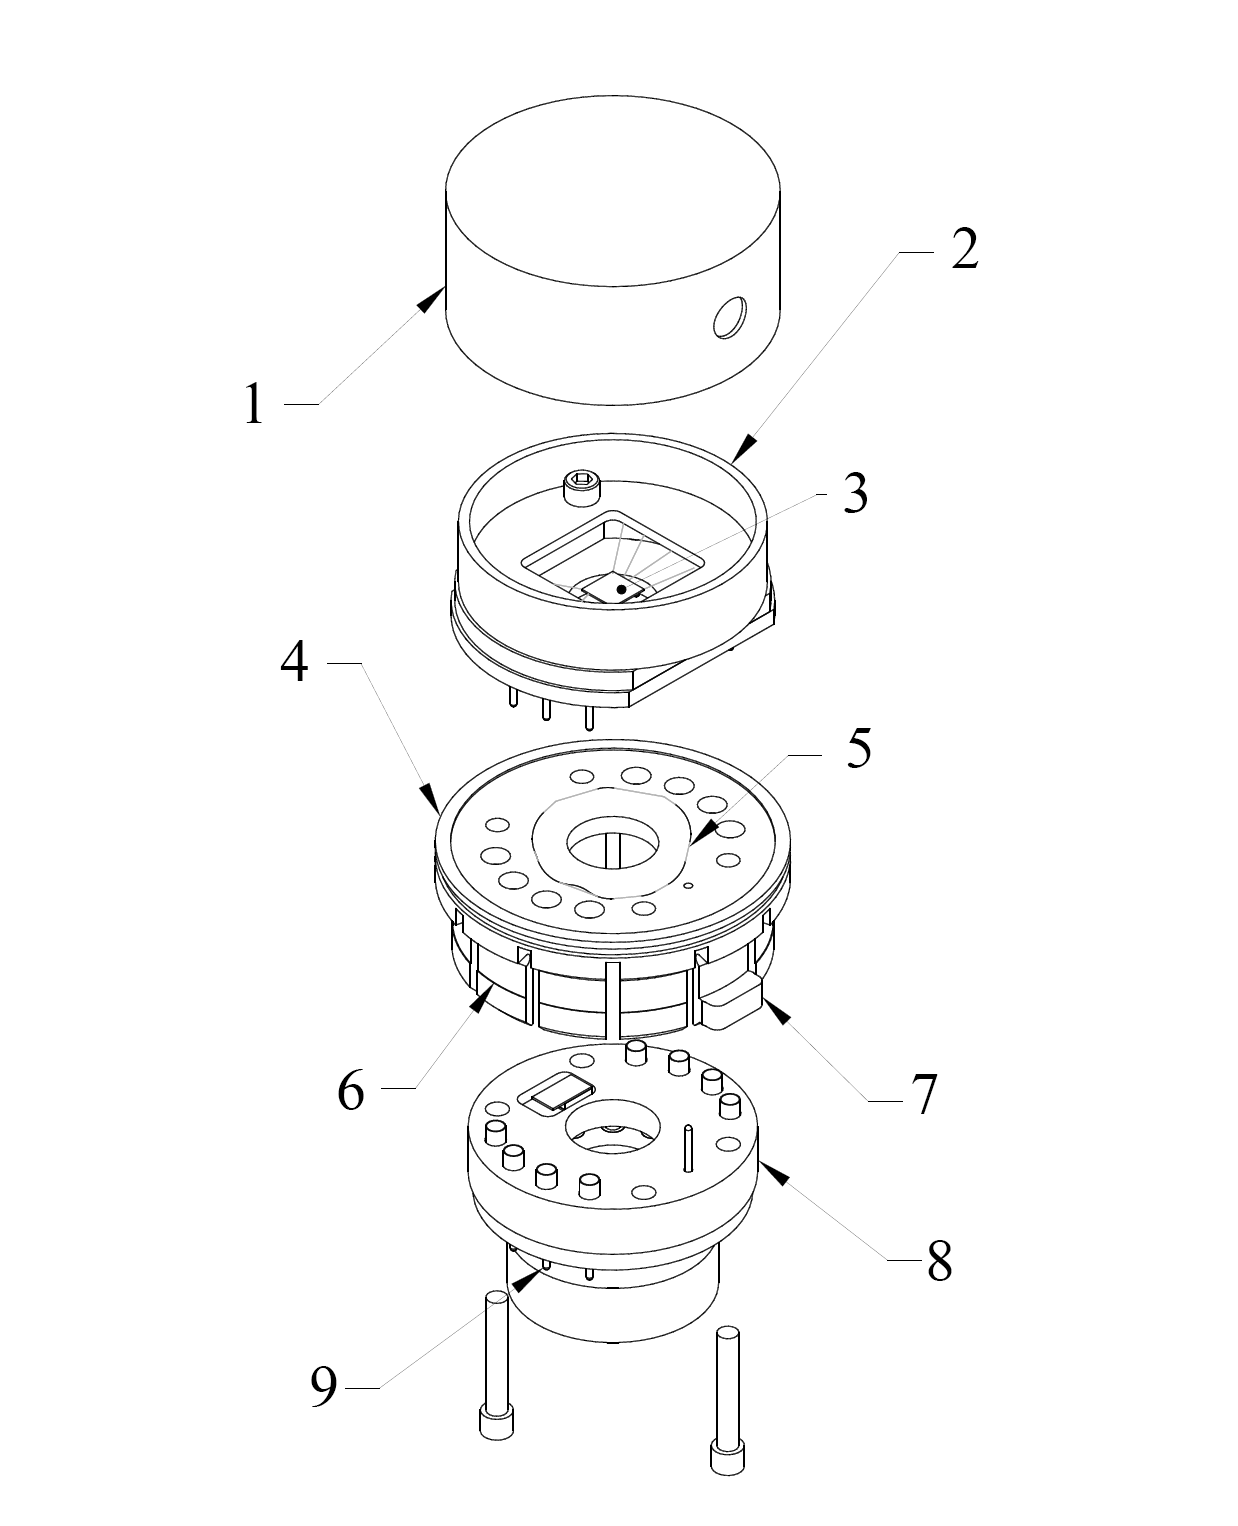
\includegraphics[width=0.99\linewidth]{5_heat_capacity_cell}
  \end{minipage}
       \caption[Схематическое изображение ячейки для измерения теплоёмкости на измерительном комплексе Quantum Design PPMS]{Схематическое изображение ячейки для измерения теплоёмкости на измерительном комплексе Quantum Design PPMS. 1 "--- защитный колпак, 2 "--- основание ячейки, 3 "--- место крепления образца, 4 "--- зажимной патрон, 5 "--- теплопроводящий гель, 6 "--- зажимы, 7 "--- индикатор положения основания ячейки, 8 "--- интерфейс, 9 "--- выходные контакты (описание дано в тексте)}
    \label{img:figure3}
\end{figure}


Описанная выше схема измерения теплоёмкости (рис. \ref{img:figure2}) реализуется в специальной ячейке, которая схематически изображена на рисунке \ref{img:figure3}. Используемая ячейка представляет собой капсулу, которая закрывается медной крышкой (1). Данная крышка выполняет  роль дополнительного теплоотвода. Крышка (1) крепится на основание (2), которое выполняет защитную функцию. На данном основании находится платформа для образца, показанная на \ref{img:figure2}. Основание (2) крепится в зажимной патрон (4), на который нанесен теплопроводящий гель (5). Зажимной патрон и основание с образцом надеваются на интерфейс (8) с помощью зажимов (6). Правильное положение крепления определяется индикатором (7). Через контакты (9) выводятся регистрируемые значения.

\subsection{Моделирование теплоёмкости}\label{sect2_4_2}
Расчётная кривая теплоёмкости получена вычислением функции Дебая с тремя дополнительными осцилляторами Эйнштейна. В теории Дебая предполагается, что атомы в кристаллической решетке являются материальными точками, которые колеблются как гармонические осцилляторы.
Каждый из этих атомов обладает 3N колебательными модами и подчиняется распределению Планка.
Теорией Дебая также предполагалось, что существует зависимость частот упругих колебаний от волнового вектора $\omega$~$=$~$\omega$(K), частота колебаний ограничивается максимальной частотой $\omega$\textsubscript{max}. При описании осцилляторов Эйнштейна подразумевается, что описываемые фононные моды квантуются, и что энергия нулевых колебаний не зависит от температуры.

Расчётная кривая теплоёмкости получена вычислением функции Дебая с тремя дополнительными осцилляторами Эйнштейна. Добавление осцилляторов Эйнштейна обсуждается в описании экспериментальных данных и обуславливает наличие мягких фононных мод в соединениях. Общая формула, по которой проводилось вычисление, имеет вид:

\begin{equation}
  \label{eq:equation2_4}
C_p(T)=9R\cfrac{T^3}{\theta_d^3}\int\limits_0^{\frac{\theta_d}{T}}\frac{e^xx^4}{(e^x-1)^2}dx+3R\sum_{i=1}^3\cfrac{e^{\frac{\theta_{e_i}}{T}}\big(\frac{\theta_{e_i}}{T}\big)^2}{\big(\frac{\theta_{e_i}}{T}-1\big)^2},
\end{equation}

где $\theta$\textsubscript{d} "--- температура Дебая, $\theta$\textsubscript{$e_i$} "--- температура соответствующего осциллятора Эйнштейна.
Осцилляторы Эйнштейна описывают дополнительный вклад в общий фононный спектр в кристаллической решетке.
Для каждого соединения дополнительные осцилляторы Эйнштейна подбирались индивидуально на основании  литературных данных и результатов, полученных во время экспериментальной работы.
\newpage
%============================================================================================================================
\section{Просвечивающая электронная микроскопия} \label{sect2_4}

Изображения структуры получены на электронном микроскопе FEI Titan 80--300 в режиме HAADF-STEM  при ускоряющем напряжении 300 кВ.
HAADF режим дает контраст по атомному номеру (зависимость Z\textsuperscript{2}).
Образец приготовлен с помощью системы фокусированного ионного пучка (FIB) на двухлучевом сканирующем микроскопе "--- FEI Helios 600.
Изображения получены при комнатной температуре на ламельке толщиной менее 100~нм и плоскости синтетического теннантита (011) Cu\textsubscript{12}As\textsubscript{4}S\textsubscript{13}.


Обработка изображений произведена в программном обеспечении atomap\cite{Nord2017}. С помощью программного обеспечения было проведено определение колонок атомов и их эллиптичность. Использовалась версия программы, которая оптимизирована для обработки кубических структур. Дополнительно был учтен дрейф и получены изображения \ref{img:mic}, показывающие величину эллиптичности для рядов атомов в направлении (011).

Изображения обработаны по следующему алгоритму:
\begin{itemize}
\item Нахождение колонок на изображении.

\item Вычитание найденных рядов, повторный поиск, введение нескольких решеток с одинокой интенсивностью.

\item Нахождение центров пиков изображения.

\item Анализ формы интенсивности от колонок, нахождение эллиптичности.

\item Учет дрейфа.
\end{itemize}

На рисунке \ref{img:mic1}а) "--- оригинальное изображение, полученное с микроскопа. На рисунке \ref{img:mic1}б) представлено обработанное изображение, на котором отмечены найденные ряды. А на рисунках \ref{img:mic1}в) и \ref{img:mic1}г) изображены значение эллиптичности для  мышьякового и медного рядов плоскости 110 соответсвенно.
Программно это определяется с помощью подбора оптимальных параметров для системы уравнений:
\begin{figure}[p!]
  \begin{minipage}[ht]{0.5\linewidth}\centering
    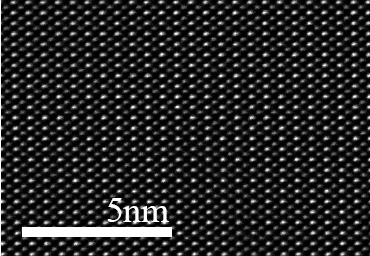
\includegraphics[width=0.7\linewidth]{mic_Figure_10} \\ а)
  \end{minipage}
  \hfill
  \begin{minipage}[ht]{0.5\linewidth}\centering
    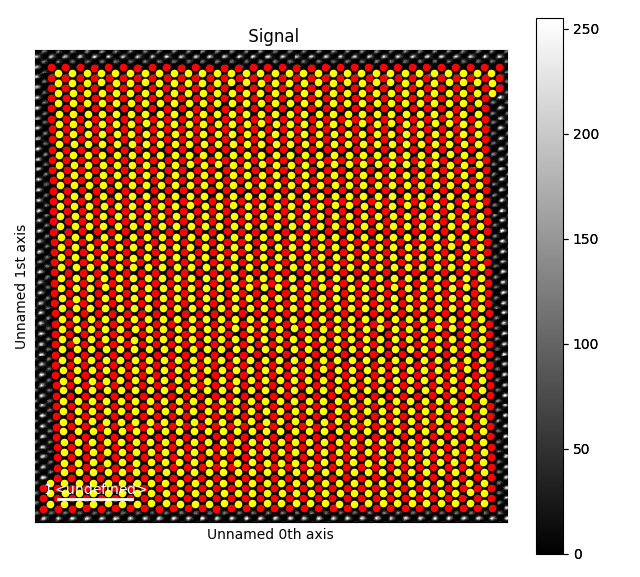
\includegraphics[width=0.9\linewidth]{mic_Figure_10_example} \\ б)
  \end{minipage}
\vfill
  \begin{minipage}[ht]{0.5\linewidth}\centering
    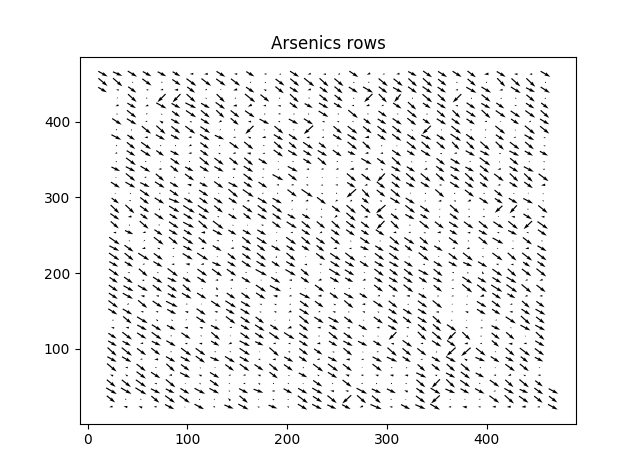
\includegraphics[width=0.9\linewidth]{mic_Figure_10_arsenic_raw} \\ в)
  \end{minipage}
  \hfill
  \begin{minipage}[ht]{0.5\linewidth}\centering
    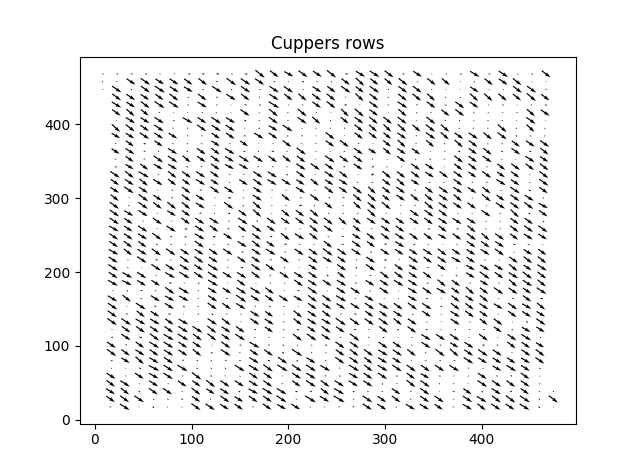
\includegraphics[width=0.9\linewidth]{mic_Figure_10_cupper_raw} \\ г)
  \end{minipage}

      \caption[Изображения структуры в режиме HAADF-STEM (а, б) и эллиптичность рядов мышьяка (в) и меди (г) синтетического теннантита Cu\textsubscript{12}As\textsubscript{4}S\textsubscript{13} в направлении (011)]{Изображения структуры в режиме HAADF-STEM (а, б) и эллиптичность рядов мышьяка (в) и меди (г) синтетического теннантита Cu\textsubscript{12}As\textsubscript{4}S\textsubscript{13} в направлении (011)}
    \label{img:mic1}
\end{figure}

\begin{equation}
  \label{eq:equation_mic}
	\begin{cases}
	I(x,y) = I_0+Aexp(-(a(x-x_0)^2-\\
	\qquad-2b(x-x_0)(y-y_0)+c(y-y_0)^2)) \\
	a=\cfrac{\cos^2\theta}{2\sigma^2_x}+\cfrac{\sin^2\theta}{2\sigma^2_y} \\
	b= - \cfrac{\sin2\theta}{4\sigma^2_x}+\cfrac{\sin2\theta}{4\sigma^2_y}\\
	c= \cfrac{\sin^2\theta}{2\sigma^2_x}+\cfrac{\cos^2\theta}{2\sigma^2_y} \\
	\end{cases},
\end{equation}
где I\textsubscript{0} "--- интенсивность фона, A "--- амплитуда центра пика, x\textsubscript{0} и y\textsubscript{0} "--- координаты центра ряда, $\sigma_x$ и $\sigma_y$ "--- стандартное отклонение, $\theta$ "--- угол поворота эллиптичности столбца.

Эллиптичность определяется по соотношению:
\begin{equation}
  \label{eq:equation_mic2}
\epsilon =
	\begin{cases}
	\cfrac{\sigma_x}{\sigma_y}, если \sigma_x > \sigma_y \\
	\cfrac{\sigma_y}{\sigma_x}, если \sigma_y > \sigma_x
	\end{cases}.
\end{equation}
\newpage
%============================================================================================================================
\section{Квантовомеханические вычисления} \label{sect2_5}
Квантовомеханические вычисления проводились в рамках теории функционала плотности. Теория функционала плотности основывается на представлении, что электронная структура определяется распределением электронной плотности.
Вычисления проводились с использованием программы VASP (Vienna Ab initio Simulation Package) \cite{Kresse1993,Kresse1994,Kresse1996}.
Эта программа позволяет проводить квантовохимические расчёты из первых принципов (ab initio) на основе функционалов метода локальной электронной плотности и обобщённого градиента в параметризации Пердью"--~Бурке"--~Эрнзерхофа (Perdew"--~Burke"--~Ernzerhof)\cite{Perdew1996}.
Вычисления основаны на методе присоединённых плоских волн, равновесная атомная геометрия зоны Бриллюэна была разбита с помощью метода Монкхоста"--~Пака (Monkhorst"--~Pack) \cite{Monkhorst_1976} на 6$\times$6$\times$6~точек. Величина энергии обрезания в расчёте равнялась 450~эВ. Оптимизация атомной структуры проводилась до тех пор, пока межатомные силы не становились меньше 0.001~эВ/${\angstrom}$.



\newpage
%============================================================================================================================
\section{Измерения намагниченности} \label{sect2_6}
Магнитные свойства образцов измерены с
помощью магнитоизмерительного комплекса
MPMS"--~XL7~EC (Quantum Design, США) с первичным преобразователем на основе СКВИДа (от англ. SQUID, Superconducting Quantum Interference Device "--- сверхпроводящий квантовый интерферометр) в диапазоне температур от 2 до 350 К и в постоянных магнитных полях напряженностью до 70 кЭ. Шаг измерения в диапазоне от $-$5 до 5~кЭ составлял 0.1~Э, при больших полях "--- 1~Э. В измерительном приборе существует возможность перевода сверхпроводящего соленоида в нормальное состояние для стабилизации поля.
Магнитоизмерительный комплекс MPMS--XL7~EC может регистрировать значения магнитного момента в диапазоне от 10\textsuperscript{-8} до 3$\cdot$см\textsuperscript{3}.
В базовой комплектации измерительный комплекс позволяет проводить магнитометрические измерения в диапазоне от 1.8 до 400~К.
Абсолютная погрешность измерения температуры составляет не более $\pm$0.5~\% в указанном выше диапазоне температур.
Погрешность измерений магнитного момента для нанокристаллических образцов и образов с постоянными магнитными моментами $\delta$\textsubscript{P~$=$~0.95}~$=$~$\pm$1.0~\%.
Для проведения измерений намагниченности образец крепили на длинную
ленту каптона внутри пластиковой трубочки, размеры которой существенно больше линейных размеров образца и градиентометра второго порядка,
состоящего из четырех измерительных витков.
Вклад от элементов крепления был полностью исключен в процессе измерения. Источником постоянного магнитного поля являлся сверхпроводящий
соленоид на основе соединения Nb\textsubscript{3}Sn.


Магнитная восприимчивость $\chi$ имеет две основные составляющие: диамагнитную, характеризующуюся магнитным моментом, возникающим на заполненных электронных оболочках, и парамагнитную, обусловленную наличием неспаренных электронов. Согласно теории Кюри"--~Вейсса магнитная
восприимчивость может быть описана выражением:

\begin{equation}
  \label{eq:equation2.1}
  \chi = \chi_{dia}+\frac{C}{T - \Theta}.
\end{equation}

Диамагнитная составляющая магнитной восприимчивости $\chi_{dia}$ найдена из графика функции
магнитной восприимчивости от обратной температуры, а температура $\Theta$ "--- из графика функции обратной магнитной восприимчивости от
температуры путём экстраполяции экспериментальной кривой.

\newpage
%============================================================================================================================
\section{Получение спектров комбинационного рассеяния} \label{sect2_6}

Спектры комбинационного рассеяния получены на спектрометре TRIAX-552, оборудованном охлаждаемым детектором Peltier TE CCD SPEC 10 (Princeton Instruments).
Были использованы: решетка 600 штрихов на мм и 50-кратная линза Mitutoyo M Plan Apo SL50 (числовая апертура 0.42).
Для получения возбуждающей линии использован аргон-ионный лазер с длинной волны 514.5 нм Spectra-Physics Stabilite 2017 и с выходной мощностью от 0.3 до 1~мВт на образце. Калибровка проведена с использованием линии спектра комбинационного рассеяния света 520.5~см\textsuperscript{-1} полированной кремниевой пластины и/или линий спектра комбинационного рассеяния неона.
Для наблюдения спектра комбинационного рассеяния света вблизи возбуждающей линии использовались 3  брэгговских фильтра.

На схеме (Рис. \ref{img:raman}) для получения спектров комбинационного света представлено расположение используемого оборудования. Инструментальная погрешность составила 4~см\textsuperscript{-1}.
\begin{figure}[p!]
  \begin{minipage}[ht]{0.99\linewidth}\centering
    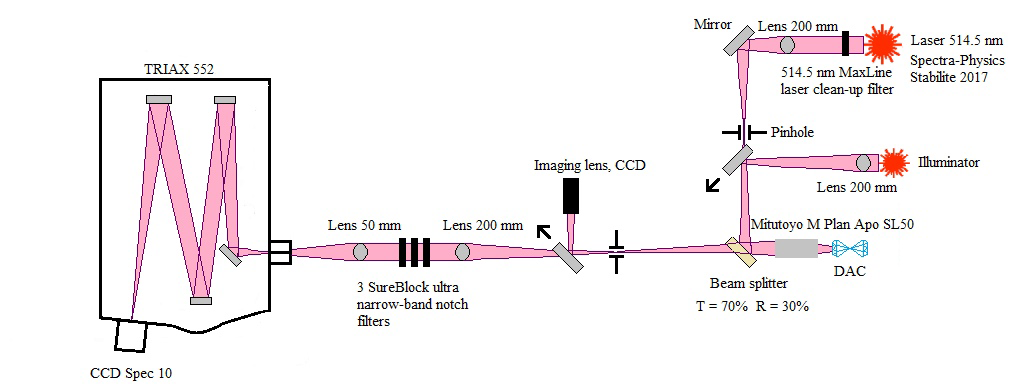
\includegraphics[width=0.99\linewidth]{raman_scheme}
  \end{minipage}


      \caption[Схематическое изображение установки для получения спектров комбинационного рассеяния]{Схематическое изображение установки для получения спектров комбинационного рассеяния}
    \label{img:raman}
\end{figure}
